\documentclass[11pt, a4paper]{article}

% --- 1. Paquetes Base y Tipografía ---
\usepackage[T1]{fontenc}
\usepackage[utf8]{inputenc}
\usepackage{lmodern} 
\usepackage{microtype} 

% --- 2. Márgenes y Espaciado ---
\usepackage[margin=1in]{geometry} 
\usepackage{setspace}
\onehalfspacing 

% --- 3. Gráficos, Matemáticas y Tablas ---
\usepackage{graphicx}
\usepackage{amsmath, amssymb, amsthm} 
\usepackage{booktabs} 
\usepackage{tabularx}
\usepackage{xcolor}

% --- 4. Enlaces interactivos ---
\usepackage[colorlinks=true, allcolors=blue]{hyperref}

% --- 5. Información del Documento ---
\title{\textbf{Título del Informe}}
\author{Mariano Fernández}
\date{\today}

\begin{document}

\maketitle
\begin{abstract}
    
\end{abstract}
\tableofcontents
\newpage

\section{Exploración y Limpieza de Datos}
\subsection{Estudio de calidad de datos}
\subsubsection{Datos faltantes por columna}

La figura \ref{fig:missing_values} muestra la cantidad de valores nulos por columna, 
se ve un porcentaje muy alto para los campos de autor ($\sim$37.7\%) y sección ($\sim$33.9\%) 
por que se pierde una parte importante del dataset al momento de sacar conclusiones de estos campos. 
También hay un $\sim$3.9\% de artículos sin cuerpo y un $\sim$0.47\% sin medio de publicación, 
los dos campos principales para este estudio.  

\begin{figure}[h]
    \centering
    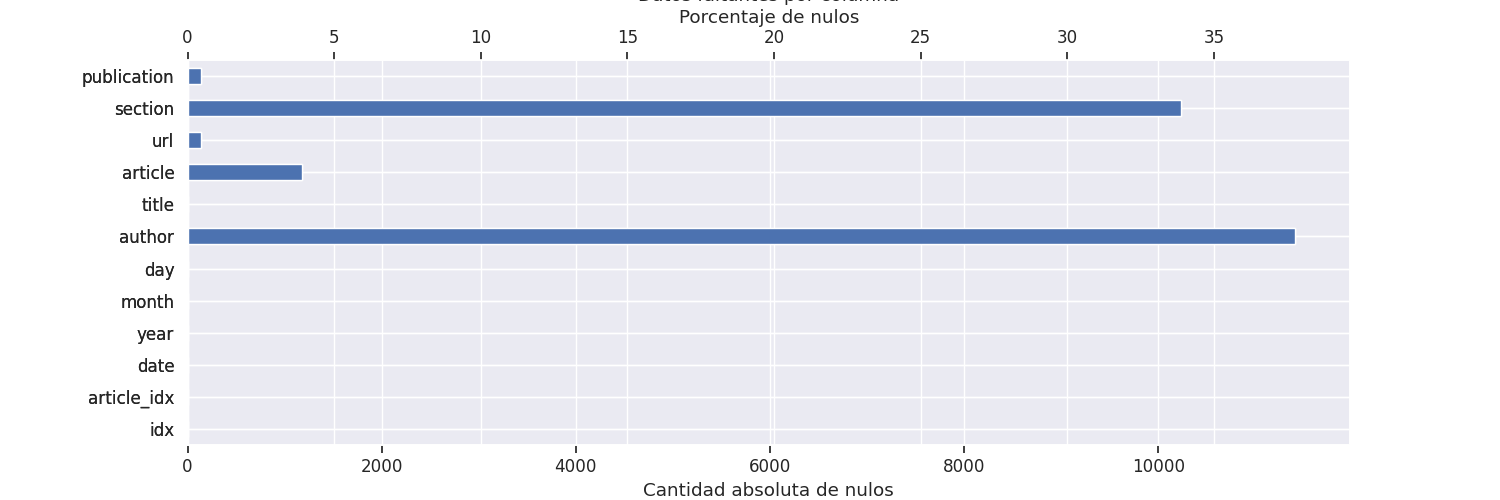
\includegraphics[width=0.8\textwidth]{figures/nulls.png}
    \caption{Cantidad de valores nulos por columna}
    \label{fig:missing_values}
\end{figure}

\subsubsection{Cantidad de artículos por medio de prensa}
La distribución de cantidad de artículos por medio de prensa se muestra en la figura \ref{fig:articles_per_publication},
se ve que un gran porcentaje de los artículos se concentran en pocos medios, 
este desbalance va a ser necesario considerarlo en una futura tarea de clasificación.

\begin{figure}[h]
    \centering
    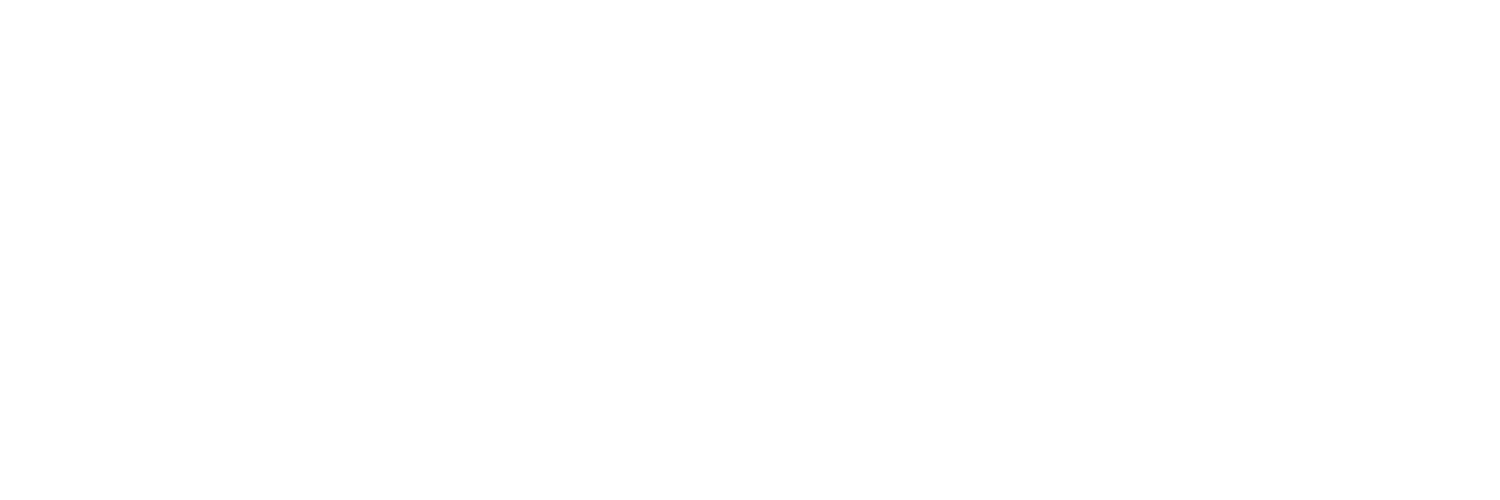
\includegraphics[width=0.8\textwidth]{figures/count_by_publication.png}
    \caption{Cantidad de artículos por medio de prensa}
    \label{fig:articles_per_publication}
\end{figure}

Los cinco medios de prensa con con mayor cantidad de artículos son:
\begin{itemize}
    \item Reuters
    \item The New York Times
    \item CNBC
    \item The Hill
    \item People
\end{itemize} 
    
El resto del análisis se hace únicamente sobre estos medios.

\subsection{Publicaciones en el tiempo}

En la figura \ref{fig:publications_over_time} se grafica la cantidad de publicaciones en el tiempo 
con una agrupando por mes, se ve un nivel mayormente estable con algunos períodos a destacar:
\begin{itemize}
    \item Mediados de 2018 -> Comienzo de 2019: Reuters dismuniyó mucho la cantidad de publicaciones
    \item Comienzos de 2019 en adelante: "CNBC" aumentó considerablemente la cantidad de publicaciones.
    \item Comienzos de 2020 en adelante: La cantidad de artículos publicados por "Reuters" 
    creció mucho en un tiempo corto y acentúa la diferencia con los otros medios.
    \item Comienzos de 2020 en adelante: No hay nuevas publicaciones de "People".
\end{itemize}

\begin{figure}[h]
    \centering
    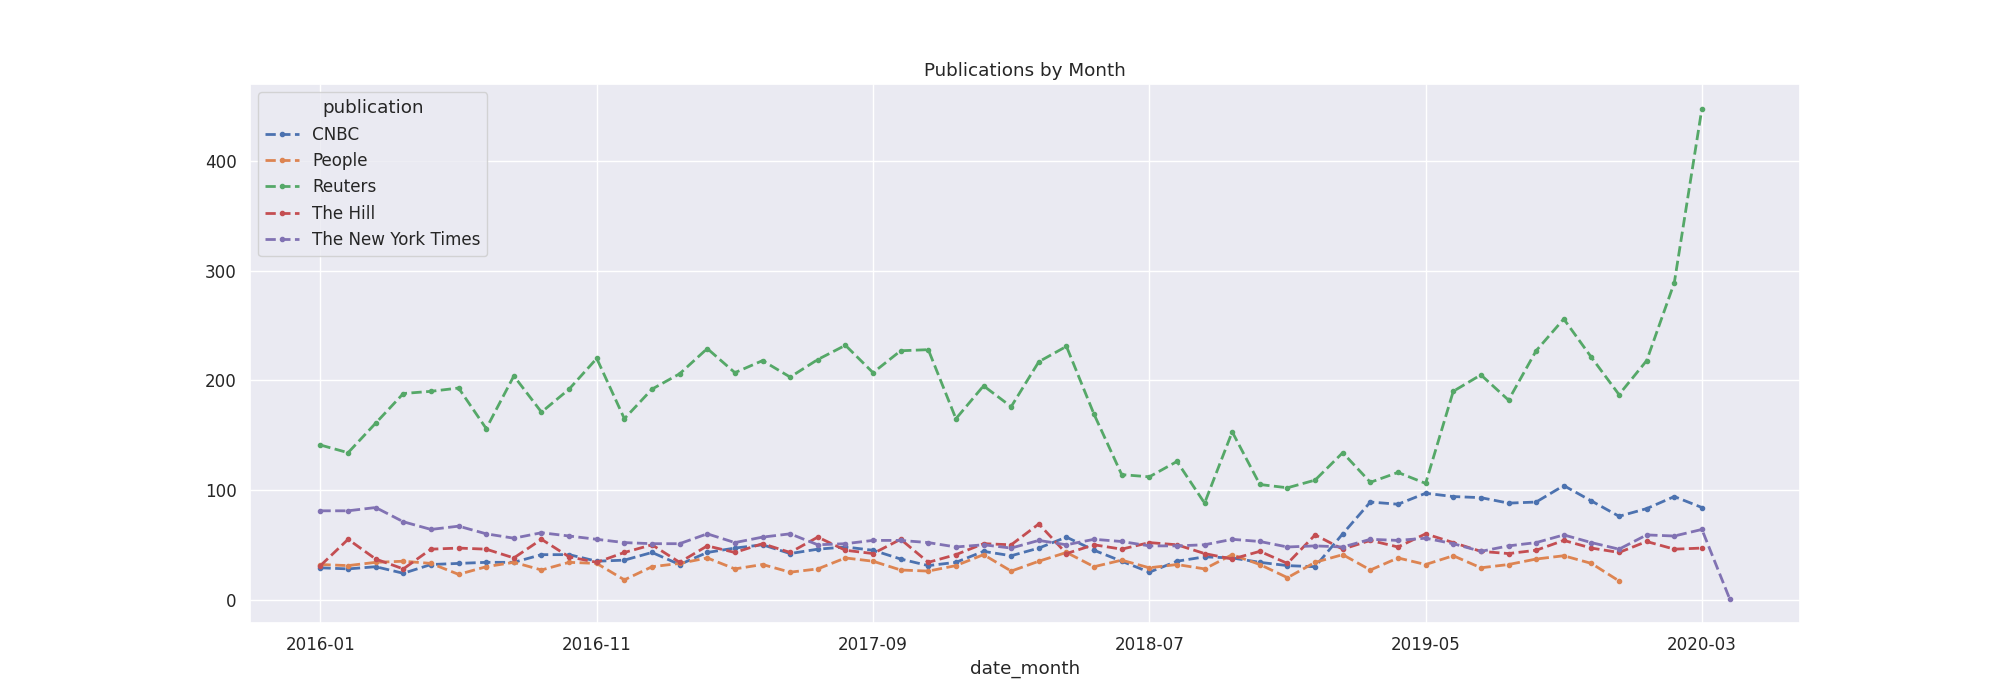
\includegraphics[width=0.8\textwidth]{figures/publications_by_month.png}
    \caption{Cantidad de publicaciones en el tiempo}
    \label{fig:publications_over_time}
\end{figure}


% \begin{figure}[h]
%     \centering
%     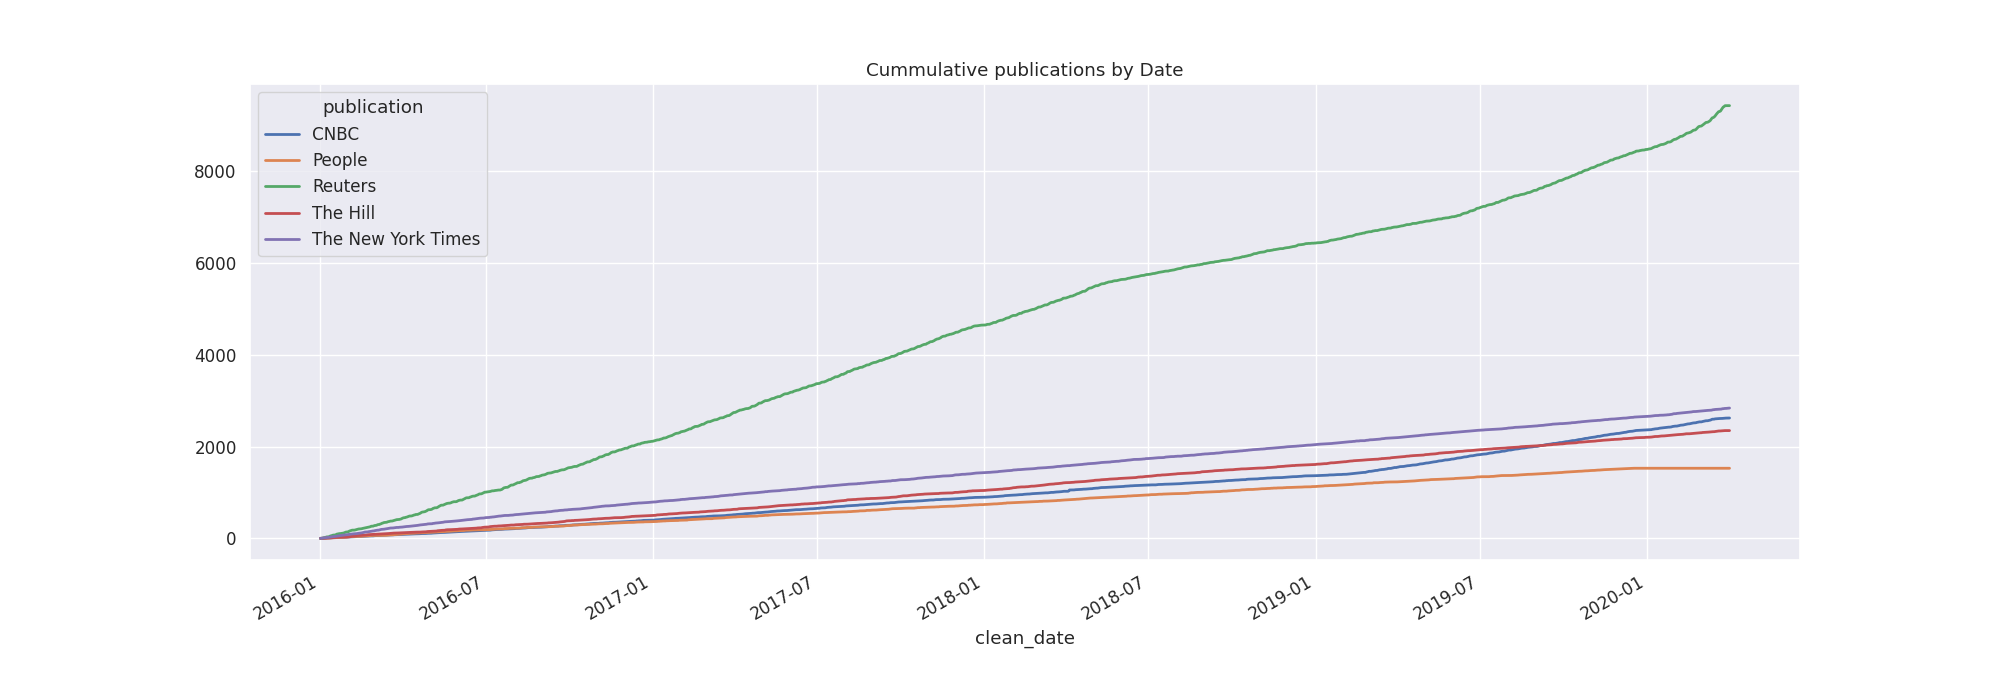
\includegraphics[width=0.8\textwidth]{figures/cummulative_publications_by_date.png}
%     \caption{Cantidad acumulada de publicaciones en el tiempo}
%     \label{fig:cummulative_publications_over_time}
% \end{figure}


\subsection{Normalización de texto}

Como paso previo al conteo de palabras se realiza una normalización del texto,
 las transformaciones aplicadas son las siguientes:\\
\begin{itemize}
    \item Eliminar primeras palabras hasta el primer salto de línea. \\
    \item Convertir texto a minúsculas.\\
    \item Eliminar símbolos\\
    \begin{itemize}
        \item Definidos previamente: \verb|"[, "\n", ",", ":", "?"|
        \item Se agregan: \\
            \verb|"(", ")", "!", ".", "'", "\"", "’",|\\
            \verb|"‘", "/", "“", "”", "]", "-", "#", ";", "xa0", "\\xa0", "\\x7f"|\\
        
        \item El método de agregar símbolos a la normalización se podría mejorar ya que fue muy manual, 
        para varios artículos muestreados aleatoreamente se imprimieron todas las palabras que 
        tuvieran símbolos no alphanuméricos y se seleccionaron los relevantes. 
        Una forma de mejorar esto podría ser usar una expresión regular para eliminar cualquier símbolo que no sea alphanumérico,
        con el riesgo de eliminar símbolos que puedan ser relevantes. 
    \end{itemize}
    \item Llenar nulos con un string vacío.
\end{itemize}


Algunos ejemplos del texto antes y después de la normalización se muestran en la tabla \ref{tab:normalization_examples}.

\begin{table}[h]
    \centering
    \small
    \begin{tabularx}{\textwidth}{@{}>{\raggedright\arraybackslash}X >{\raggedright\arraybackslash}X >{\raggedright\arraybackslash}X >{\raggedright\arraybackslash}X@{}}
        \toprule
        \textbf{Title} & \textbf{Clean Title} & \textbf{Article} & \textbf{Clean Article} \\
        \midrule
        'Sonic the Hedgehog' faces video game adaptation box office curse & sonic the hedgehog faces video game adaptation box office curse & Hollywood has long tried to capitalize on the financial success and cultural relevance of video game & hollywood has long tried to capitalize on the financial success and cultural relevance of video game \\
        Norway sets world record with electric cars sold last year \textbar{} TheHill & norway sets world record with electric cars sold last year \textbar{} thehill & Norway set a new world record last year after nearly a third of all its new car sales were electric, & norway set a new world record last year after nearly a third of all its new car sales were electric \\
        BRIEF-FS Bancorp Inc announces commencement of public offering of common stock & brief fs bancorp inc announces commencement of public offering of common stock & Sept 5 (Reuters) - Fs Bancorp Inc * FS Bancorp Inc announces commencement of public offering of comm & sept 5 reuters fs bancorp inc * fs bancorp inc announces commencement of public offering of comm \\
        Pawnee Nation Sues Oklahoma Oil Companies in Tribal Court Over Earthquake Damage & pawnee nation sues oklahoma oil companies in tribal court over earthquake damage & OKLAHOMA CITY — A Native American tribe here has filed a lawsuit in its own tribal court system accu & oklahoma city — a native american tribe here has filed a lawsuit in its own tribal court system accu \\
        Turkey says agreed with Russia on details of Idlib ceasefire: Anadolu & turkey says agreed with russia on details of idlib ceasefire anadolu & ANKARA (Reuters) - Turkish and Russian officials have agreed on the details of a ceasefire in northw & ankara reuters turkish and russian officials have agreed on the details of a ceasefire in northw \\
        \bottomrule
    \end{tabularx}
    \caption{Ejemplos de texto antes y después de la normalización}
    \label{tab:normalization_examples}
\end{table}

\subsection{Elección de campos de texto}

En principio ambos el título y el cuerpo del artículo pueden contener información relevante a usar 
en una futura tarea de clasificación, pero esto va a depender del estudio que se realice. 
Por ejemplo si se combinan ambos en un campo solo para realizar tareas como conteo de 
palabras el título no va a agregar mucha información porque va a ser un porcentaje muy chico del total. 
Pero por otro lado parece razonable pensar que diferentes medios tengan "tipos" de títulos diferentes, 
por lo dependiendo del modelo podría ser información útil a agregar. Para este caso se decide usar solo 
el cuerpo del artículo para el análisis de palabras por simplcidad.

\subsection{Pistas del medio de prensa en el texto}
Para estudiar si hay información que identifique muy fácilmente el medio de publicación 
de un artículo lo primero fue tomar muestras random de algunos artículos para cada medio y
 visualizar el comienzo y final del texto. Con unos pocos ejemplos ya se pueden sacar varias conclusiones:

\begin{enumerate}
    \item Todos los artículos de \textit{The Hill} terminan de la misma forma. Ejemplo:
    \begin{quote}
        \texttt{...view the discussion thread the hill 1625 k street nw suite 900 ... 
            capitol hill publishing corp a subsidiary of news communications inc}
    \end{quote}
    
    \item La mayoría de los artículos de \textit{Reuters} terminan de la misma forma listando las personas que contribuyeron. Ejemplo:
    \begin{quote}
        \texttt{...reporting by kylie maclellan writing by elizabeth piper editing by paul sandle}
    \end{quote}
    
    \item Todos los artículos de \textit{Reuters} 
        parecen comenzar con el patrón \verb|<lugar> y/o <fecha> - reuters|. Ejemplos:
    \begin{enumerate}
        \item \texttt{may 10 reuters...}
        \item \texttt{kuala lumpur march 13 reuters...}
        \item \texttt{london reuters...}
    \end{enumerate}
    
    \item Parece haber un error en la data: varios artículos etiquetados como \textit{CNBC} tienen el mismo comienzo y final que se ve en los artículos de \textit{Reuters}. Ejemplos:
    \begin{enumerate}
        \item \texttt{bucharest aug 13 reuters ... 
            reporting by radu marinas and alicja ptak editing by alexandra hudson}
        \item \texttt{hong kong july 15 reuters ... 
            reporting by julie zhu in hong kong writing by jennifer hughes editing by jane merriman}
    \end{enumerate}
\end{enumerate}

Para verificar que no hubieran urls que identifiquen el medio en el texto se utilizó 
la siguiente expresión regular \verb!r'(?:https?://|www\.)[^\s]+'! 
aplicada al cuerpo del texto sin normalizar, 
luego se agrupó por dominio para visualizar cuales aparecían en más de un 1\% de los artículos por medio, 
no se encontraron resultados destacables.

Similarmente, para el caso de emails se utilizó una expresión regular para encontrar emails
 y tags que identifiquen el medio, en este caso se aplicó la expresión
  \verb|r'\S*@[a-zA-Z0-9.-]+\S*'| sobre el cuerpo del artículo normalizado. A destacar:
  \begin{itemize}
  \item @cnbc aparece en 2.36\% de los artículos del medio.
  \item @thehill aparece en 1.83\% de los artículos del medio.
  \item @nytimes (7.68\%) y @nytopinion (3.20\%)
  \end{itemize}

Medio de prensa: El caso más relevantes son las menciones del mismo medio, 
un gran porcentaje de los artículos menciona al medio en el cuerpo, el detalle
se muestra en la tabla \ref{tab:pistas_medios}, el caso de Reuters y The Hill 
se explica por el uso de plantillas ya detectadas.

\begin{table}[hbt!]
    \centering
    \caption{Menciones del medio de prensa en el cuerpo del artículo}
    \label{tab:pistas_medios}
    \begin{tabular}{lrl}
        \toprule
        \textbf{Medio de Prensa} & \textbf{ "Pistas" (\% de artículos con al menos una mención)} \\
        \midrule
        CNBC & cnbc (33.89\%), madcap@cnbc (2.21\%) \\
        People & people (66.62\%), peopletv (2.23\%), peoplestyle (1.70\%) \\
        Reuters & reuters (88.58\%) \\
        The Hill & the hill (99.40\%), @thehill (1.02\%) \\
        The New York Times & the new york times (16.97\%) \\
        \bottomrule
    \end{tabular}
\end{table}


A partir de estos resultados la primera decisión a tomar es que hacer con los artículos de CNBC
que parecen tener un error de anotación, ya que tienen el mismo patrón que los artículos de Reuters.
Cambiar el medio de publicación a Reuters puede ser una opción pero introduce un riesgo grande
de que no todos los artículos afectados sean de Reuters, si se estuviera trabjando con un 
conjuntos de datos más pequeño tendría sentido dedicar más tiempo a este análisis pero para 
este caso "Reuters" ya es el medio con más artículos por lo que se decide eliminar los artículos de
CNBC que tengan el patrón de Reuters, este es el camino más seguro para evitar introducir un sesgo 
incorrecto.

Luego la decisión de eliminar estos patrones depende de cual es el objetivo final, 
si a partir de estos datos se va a intentar obtener un modelo de clasificación 
es necesario que los datos de entrenamiento tengan una distrubución lo más cerca 
posible a la distribución real donde se va a aplicar el modelo. 
No eliminar estos patrones simplifican mucho el problema pero asumen que esto no va a cambiar, 
lo que haría que el modelo tenga una capacidad de generalización muy baja, por ejemplo 
si un día reuters cambia el modelo perdería la capacidad de clasificar correctamente. 
Para este estudio se decide eliminar los patrones más evidentes, en particular se usan las siguientes
expresiones regulares para eliminar esa sección del texto.
\begin{itemize}
    \item \verb|r'(view the discussion thread  )?the hill 1625 k street  nw suite 900.*'|
    \item \verb|r'reporting by.*'|
    \item \verb|r'^[a-z\s\d]{5,30}reuters'|
    \item \verb|r'@cnbc'|
    \item \verb|r'@thehill'|
    \item \verb|r'@nyt\w*'|
\end{itemize}

\subsection{Restricción de los datos}

Dado el análisis temporal realizado en las sección 1.2 filtraría los datos posteriores a 2020, 
ya que dejan de haber publicaciones de "People". 
Graficando la cantidad de publiciones para los diferentes meses del ano no hay una diferencia 
clara para ninguno de los medios, si se diera el caso que no hayan o hayan menos publicaciones 
para un medio en algún momento del ano podría haber sido útil filtrar ese período.

Si hay secciones temáticas que publican solo algunos medios y otros no se repite una discusión 
similar a que patrones de los datos es necesario eliminar o reducir su impacto, 
si no se restringe a temáticas sobre las que escriben todos los medios el modelo podría aprender 
un sesgo de que cierta temática está asociada a cierto medio pero si eso cambia en el futuro o 
los datos de entrenamiento no estaban completos la precisión del modelo va a ser baja.

\section{Conteo de Palabras y Visualizaciones}
\subsection{Palabras más frecuentes}

La figura \ref{fig:most_common_words_heatmap} es un mapa de calor de las 5 palabras 
más frecuentes para cada medio de prensa (hay mucho solapamiento entre los medios), 
en general todas son artículos que no aportan información relevante, por ejemplo "the", "to", "of", "a", "and", etc.
Y son frecuentes en todos los medios, con algunas diferencias.

En la figura \ref{fig:most_common_words_no_stopwords_heatmap} 
se vuelve a realizar el conteo de palabras pero eliminando las "stopwords" del idioma inglés con la
librería nltk, esto mejora mucho la visualización y ya se pueden tomar conslusiones interesantes,
por ejemplo "The Hill" tiene muchas más menciones de "Trump" que los otros medios.

Algo se puede ver en la figura \ref{fig:most_common_words_no_stopwords_heatmap} pero 
sería interesante una visualización que muestre las palabras que son muy frecuentes 
en un medio pero no en los otros.

% \begin{figure}[h]
%     \centering
%     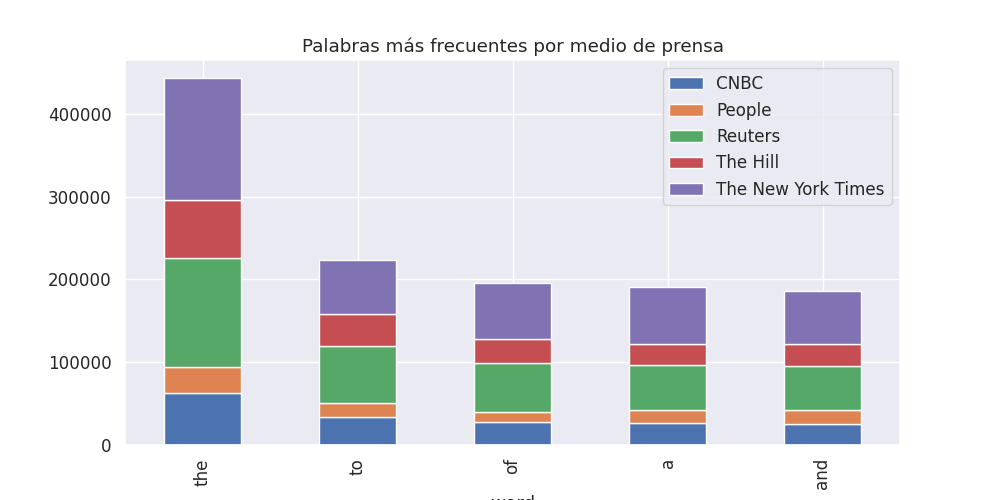
\includegraphics[width=0.8\textwidth]{figures/most_common_words.png}
%     \caption{Palabras más frecuentes}
%     \label{fig:most_common_words}
% \end{figure}

\begin{figure}[h]
    \centering
    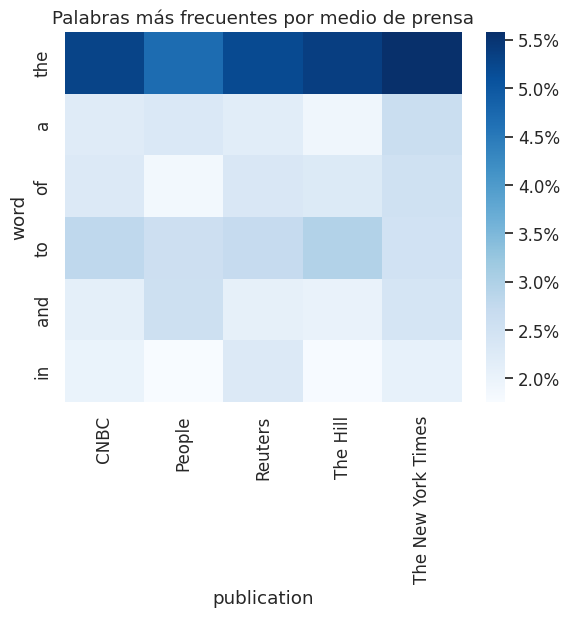
\includegraphics[width=0.8\textwidth]{figures/most_common_words_heatmap.png}
    \caption{Palabras más frecuentes por medio de prensa}
    \label{fig:most_common_words_heatmap}
\end{figure}

% \begin{figure}[h]
%     \centering
%     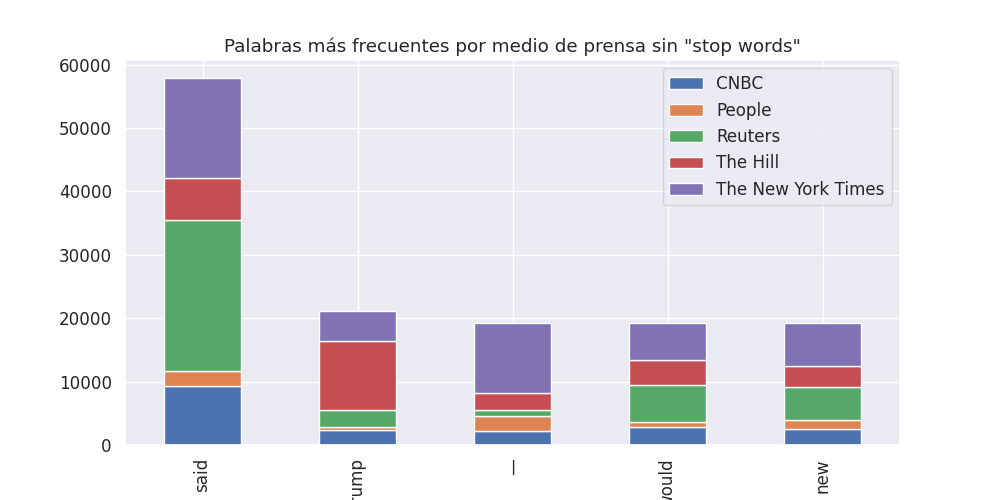
\includegraphics[width=0.8\textwidth]{figures/most_common_words_no_stopwords.png}
%     \caption{Palabras más frecuentes (sin stopwords)}
%     \label{fig:most_common_words_no_stopwords}
% \end{figure}

\begin{figure}[h]
    \centering
    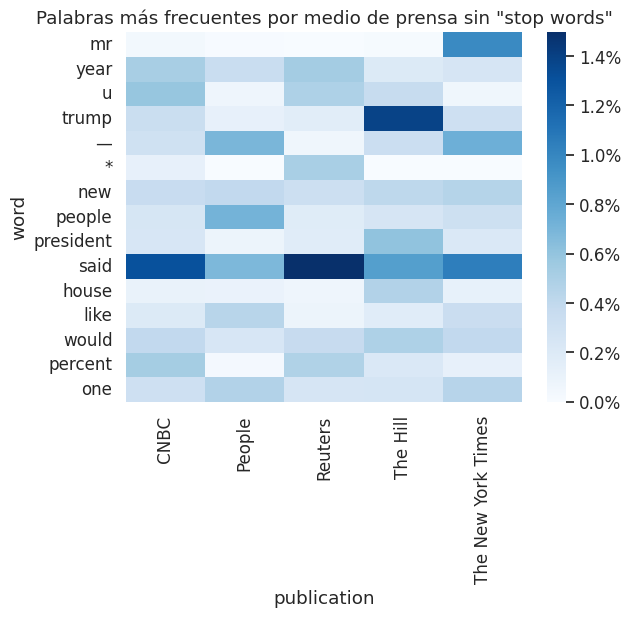
\includegraphics[width=0.8\textwidth]{figures/most_common_words_no_stopwords_heatmap.png}
    \caption{Palabras más frecuentes (sin stopwords)}
    \label{fig:most_common_words_no_stopwords_heatmap}
\end{figure}

\subsection{Medios con mayor cantidad de palabras}


En la figura \ref{fig:word_count_by_publication} se muestra la cantidad total 
de palabras publicadas por medio de prensa, un punto muy interesante es que "Reuters" tiene 
cantidad similar "The New York Times" que tiene mucho menos artículos publicados.
Esto último se puede visualizar mejor en la figura \ref{fig:word_count_by_publication_normalized} 
donde se normaliza la cantidad de palabras por la cantidad de artículos publicados por medio, 
esto nos da una idea del tamaño promedio de los artículos por medio.
\begin{figure}[h]
    \centering
    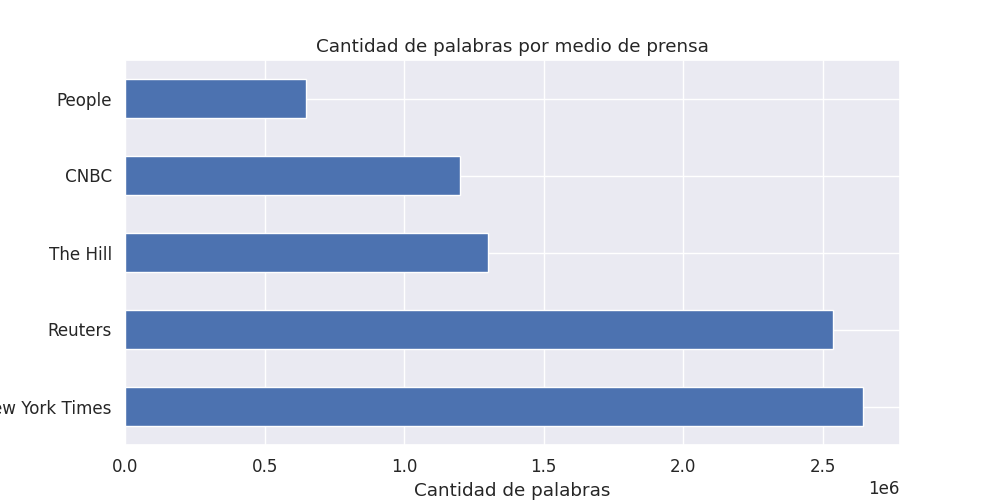
\includegraphics[width=0.8\textwidth]{figures/word_count_by_publication.png}
    \caption{Cantidad de palabras por medio de prensa}
    \label{fig:word_count_by_publication}
\end{figure}

\begin{figure}[h]
    \centering
    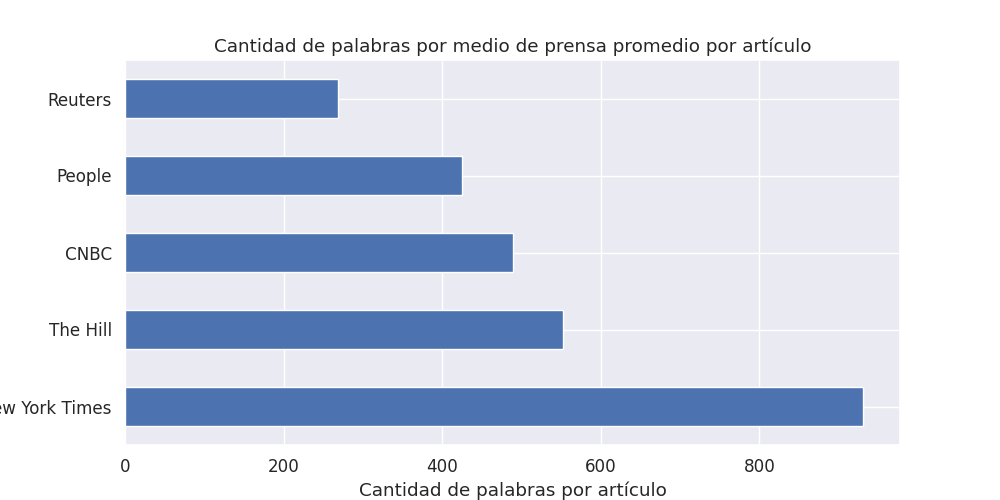
\includegraphics[width=0.8\textwidth]{figures/word_count_by_publication_normalized.png}
    \caption{Cantidad de palabras por medio de prensa normalizado por cantidad de artículos}
    \label{fig:word_count_by_publication_normalized}
\end{figure}

\subsection{Menciones entre medios}

Visualizando las menciones entre medios de prensa se ve un problema importante, la palabra "People" es muy común
por lo que en las figuras \ref{fig:mentions_matrix} y \ref{fig:mentions_graph} se ve que "People" tiene muchas menciones
de todos los medios. Una posible forma de mitigar este problema es hacer el matching antes de pasar el texto a minúsculas,
ya que los casos de "People" con mayúscula que no refieran al medio de prensa deberían ser solo al comienzo de una oración, 
y esos también se podrían filtrar con expresiones regulares.

\begin{figure}[h]
    \centering
    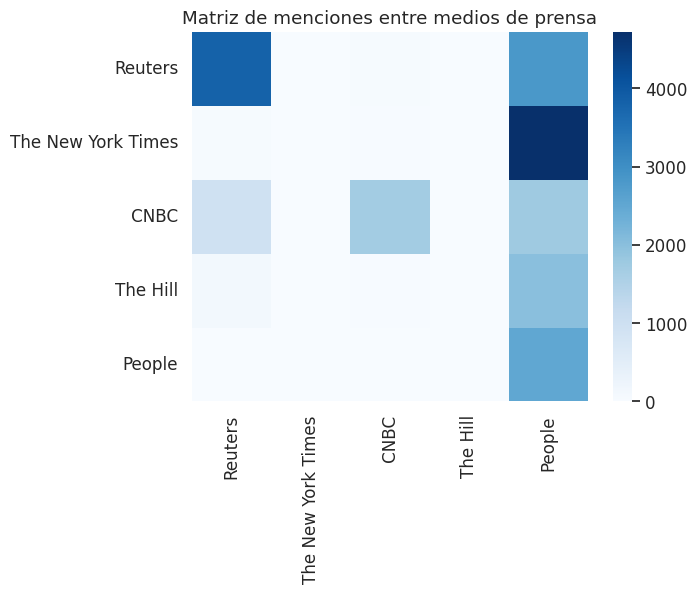
\includegraphics[width=0.8\textwidth]{figures/mentions_matrix.png}
    \caption{Matriz de menciones entre medios de prensa}
    \label{fig:mentions_matrix}
\end{figure}

\begin{figure}[h]
    \centering
    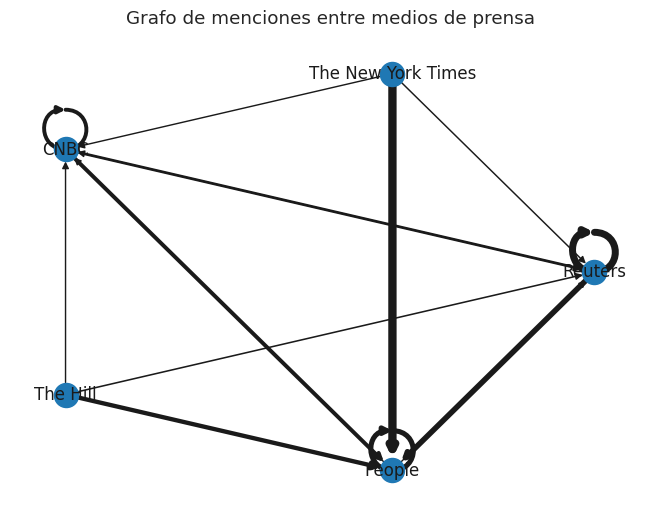
\includegraphics[width=0.8\textwidth]{figures/mentions_graph.png}
    \caption{Grafo de menciones entre medios de prensa}
    \label{fig:mentions_graph}
\end{figure}


\subsection{Posibles preguntas}
Algunas preguntas interesantes para seguir explorando los datos podrían ser:

- ¿Hay diferencias en la "complejidad" de los artículos 
    entre medios de prensa? \\
    Se podría medir la cantidad de palabras por artículo, 
    o el tipo de palabras utilizadas.

- ¿Los medios tienen un sentimiento predominante asociado a noticias
    de ciertas temáticas? \\
    Una forma sería contar la cantidad de palabras positivas / negativas 
    por tema y medio de prensa, aunque esto es un método muy simple, 
    para llegar a buenos resultados lo ideal sería un modelo de
    análisis de sentimiento.

- ¿Es viable detectar el medio de prensa de un artículo a partir de la
    frecuencia de las palabras usadas? \\
    Una forma sería definir como features a la frecuencia de las palabras 
    usadas y tomar eso como entrada del modelo. 

\end{document}